% Font size, paper type
\documentclass[12pt]{article}
% Aesthetic margins
\usepackage[margin=1in]{geometry}
% Core math packages,
% Mathtools loads amsmath, and amsmath gives basic math symbs
% Amsfonts & amssymb are misc. symbols you might need
\usepackage{mathtools, amsfonts, amssymb}
% Links in a pdf
\usepackage{hyperref}
% Use in pictures, graphs, and figures
\usepackage{graphicx}
% Header package
\usepackage{fancyhdr}
% Underlining with line breaks
\usepackage{ulem}
% Adjust accordingly given warning messages
\setlength{\headheight}{15pt}
% So we can more easily format text with pictures
\usepackage{float}

% Sets footer
\pagestyle{fancy}
% Removes default footer style
\fancyhf{}

\rhead{
  Shengdong Li
  Calc 3
}

\rfoot{
  Page \thepage
}

% Makes links look more appealling
\hypersetup{
    colorlinks=true,
    linkcolor=blue,
    filecolor=magenta,      
    urlcolor=cyan,
}

% \usepackage{indentfirst}

\begin{document}
\title{Problem 1 = $\int_{0}^{1}\cos\left(2x\right)dx$}
\author{by Shengdong Li}
\date{3 December 2020}
\maketitle

\section{Taylor via Maclaurin}
\begin{align}
  \intertext{To begin solving the taylor series for this problem, I decided to just use the maclaurin series and center it at $0$, since we already know the shortcut to get to $\cos(x^2)$ from knowing the formula for $\cos(x)$. Also, it encompasses the left bound, $0$ }
  \cos\left(x\right)                            & =\sum_{n=0}^{\infty}\frac{\left(-1\right)^{n}\cdot x^{2n}}{\left(2n\right)!}                                                                                                                     \\
  \intertext{We can plugin $x^2$ for $x$}
  \cos\left(x^{2}\right)                        & =\sum_{n=0}^{\infty}\frac{\left(-1\right)^{n}\cdot\left(x^{2}\right)^{2n}}{\left(2n\right)!}                                                                                                     \\
  \cos\left(x^{2}\right)                        & =\sum_{n=0}^{\infty}\frac{\left(-1\right)^{n}\cdot x^{4n}}{\left(2n\right)!}                                                                                                                     \\
  \intertext{From here, I chose to go up to the fourth degree taylor polynomial, so that it is as accurate as possible without being impossible to calculate by hand. One point to note here is that because the summation notation of the taylor series skips over the $0$s, to get to the $4$th degree polynomial we just need to go up to $n=1$}
  T_{4}\left(x\right)                           & =\frac{\left(-1\right)^{\left(0\right)}\cdot x^{4\left(0\right)}}{\left(2\left(0\right)\right)!}+\frac{\left(-1\right)^{\left(1\right)}\cdot x^{4\left(1\right)}}{\left(2\left(1\right)\right)!} \\
                                                & =1-\frac{1}{2}x^{4}                                                                                                                                                                              \\
  \intertext{We can then find the integral of this function from $0$ to $1$}
  \int_{0}^{1}\left(1-\frac{1}{2}x^{4}\right)dx & =\int_{0}^{1}dx-\frac{1}{2}\int_{0}^{1}x^{4}dx                                                                                                                                                   \\
                                                & =\left[x\right]_{0}^{1}-\frac{1}{2}\left[\frac{1}{5}x^{5}\right]_{0}^{1}                                                                                                                         \\
                                                & =\left(\left(1\right)-\left(0\right)\right)-\frac{1}{10}\left(\left(1\right)^{5}-0\right)                                                                                                        \\
                                                & =1-\frac{1}{10}
  \intertext{This gives us a final value of}
  \Aboxed{                                      & =\frac{9}{10}}
\end{align}
\section{Riemann Sums via Simpson's}
\begin{align}
  \intertext{For Riemann Sums, I decided to use Simpson's Rule, since it's the most accurate out of all the methods, with $n=4$, matching the number of terms in $T_4(x)$}
  \Delta x & =\frac{1-0}{4}=\frac{1}{4}                                                                                                                                       \\
  S_{4}    & =\frac{\left(\frac{1}{4}\right)}{3}\left(f\left(0\right)+4f\left(\frac{1}{4}\right)+2f\left(\frac{1}{2}\right)+4f\left(\frac{3}{4}\right)+f\left(1\right)\right) \\
           & =\frac{\left(\frac{1}{4}\right)}{3}\left(1+4\left(0.998\right)+2\left(.967\right)+4\left(.846\right)+\left(.540\right)\right)                                    \\
  \Aboxed{ & =.904}
\end{align}

\section{Observations}
Comparing the results, the two methods gave very close answers, within $0.005$ of each other. In terms of the terms, $T_4(x)$ of $\cos(x^2)$ only had $2$ terms, while Riemann had a full $5$ strips, so it's hard to say which one is better in this context.

Observing the graphs of the two methods, we can see that
\begin{figure}[H]
  \begin{center}
    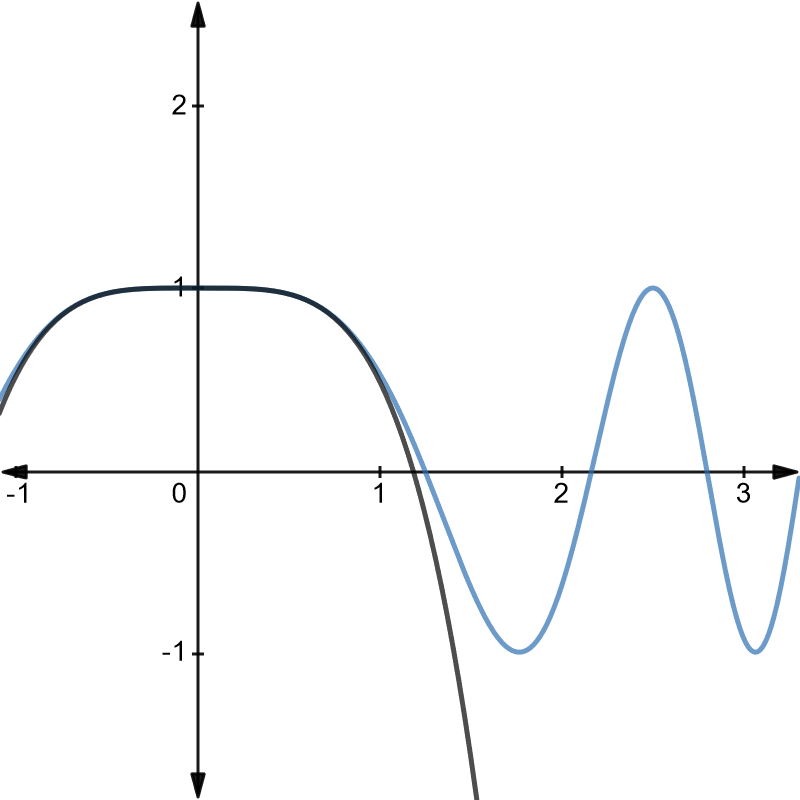
\includegraphics[scale=.3]{taylor.png}
    \caption{\textit{Picture of taylor function.} Desmos link \href{https://www.desmos.com/calculator/r4zur75mvp}{\textcolor{blue}{here}}}
  \end{center}
\end{figure}

\begin{figure}[h]
  \begin{center}
    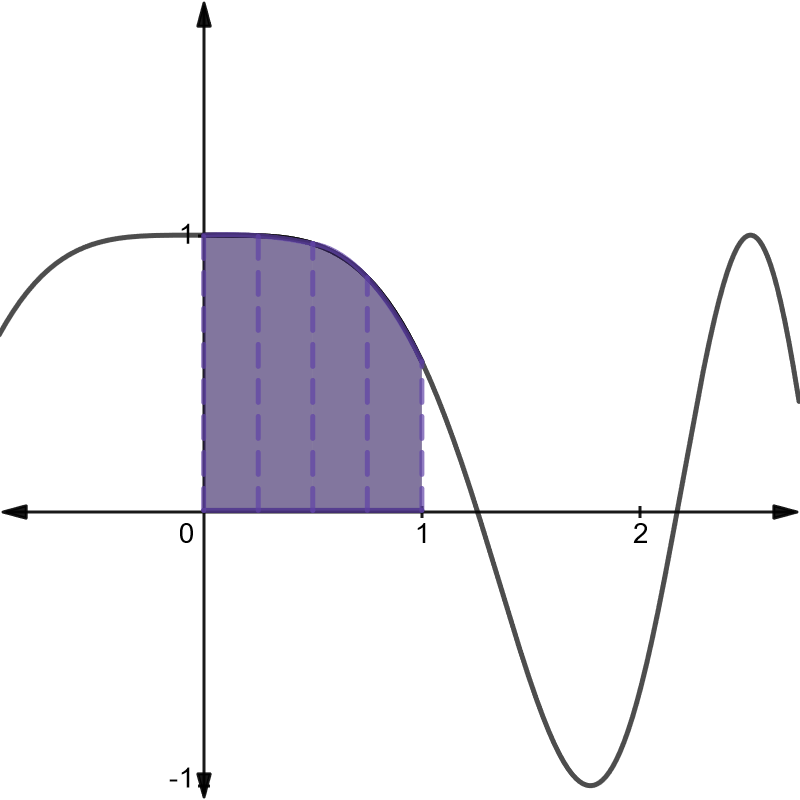
\includegraphics[scale=.3]{riemann.png}
    \caption{\textit{Picture of riemann sum.} Desmos link \href{https://www.desmos.com/calculator/zrvlosytaf}{\textcolor{blue}{here}}}
  \end{center}
\end{figure}

Both approximations of $\cos(x^2)$ are very close. However, if we kept going and expanded the bounds from $0$ to $2$, then the taylor representation would rapidly start to become very inaccurate compared to Simpson's.

Therefore, especially for a series like $\cos(x^2)$, which has so many bends, Riemann might be more accurate and more convenient if the bounds were slightly larger.
% Remember to use \ldots
\end{document}